\documentclass[10pt]{article}
\usepackage{amsmath,amsthm}
\usepackage{amssymb}
\usepackage{anysize}
\usepackage{listings}
\usepackage{graphicx}

\usepackage[italian]{babel}

\usepackage{booktabs}

\usepackage{thmtools}
\usepackage[italian]{cleveref}
\usepackage{nameref}

\usepackage{siunitx}

\usepackage{xcolor}

\definecolor{Blue}{rgb}{0.2,0.2,0.9}
\definecolor{Green}{rgb}{0,0.6,0}
\definecolor{Gray}{rgb}{0.5,0.5,0.5}
\definecolor{Purple}{rgb}{0.58,0,0.82}
\definecolor{background}{rgb}{0.98,0.98,0.95}

\lstdefinestyle{mystyle}{
    backgroundcolor=\color{background},   
    commentstyle=\color{Green},
    keywordstyle=\color{Blue},
    numberstyle=\tiny\color{Gray},
    stringstyle=\color{Purple},
    basicstyle=\ttfamily\footnotesize,
    breakatwhitespace=false,         
    breaklines=true,                 
    captionpos=b,                    
    keepspaces=true,                 
    numbers=left,                    
    numbersep=5pt,                  
    showspaces=false,                
    showstringspaces=false,
    showtabs=false,                  
    tabsize=2
}


\lstset{style=mystyle}


%%% OPERATORS
    \DeclareMathOperator{\pr}{Pr}
\DeclareMathOperator{\erf}{erf}
\DeclareMathOperator{\Beta}{Beta}
\DeclareMathOperator{\Ga}{Ga}
\DeclareMathOperator{\Exp}{Exp}
\DeclareMathOperator{\Unif}{Unif}
\DeclareMathOperator{\Cov}{Cov}
\DeclareMathOperator{\corr}{corr}
\DeclareMathOperator*{\argmax}{argmax}
\DeclareMathOperator*{\argmin}{argmin}
\DeclareMathOperator{\NLL}{NLL}
%%%

%% MATH MISC
\renewcommand{\vec}[1]{\boldsymbol{#1}}
\newcommand{\tens}[1]{\mathsf{#1}}
\newcommand{\pd}[2]{\frac{\partial #1}{\partial #2} }
\newcommand{\HALF}{\frac{1}{2}}
\newcommand{\DS}{\displaystyle}
%% TEXT
\newcommand{\im}[1]{\textsc{#1}}
%% LOGIC
\newcommand{\et}{\wedge}
\newcommand{\orr}{\vee}
\newcommand{\cond}{\mid}
%% PARENTESIS
\newcommand{\lp}{\left}
\newcommand{\rp}{\right}
\newcommand{\pare}[1]{
	\ensuremath{\left(#1\right)}
}
\newcommand{\spare}[1]{
	\ensuremath{\left[#1\right]}
}
%% DERIVATE
\newcommand{\deriv}[3][]{
	\ensuremath{\frac{d^{#1}{#2}}{d{#3}^{#1}}}
}
\newcommand{\pderiv}[3][]{
	\ensuremath{\frac{\partial^{#1}{#2}}{\partial{#3}^{#1}}}
}
%% TALE CHE
\newcommand{\tc}{\ensuremath{\;\text{t.c.}\;}}
\newcommand{\tcq}{\ensuremath{\quad\text{t.c.}\quad}}
%% TEXT IN MATH
\newcommand{\MLE}{\ensuremath{\text{MLE}}}
%% NAMED CREF
\newcommand{\Crefn}[1]{\Cref{#1} (\nameref{#1})}

%%%%%%%%%%%%%%%%%%%%%%%%%%%%%%%%%%%%%%%%%%%%%%%%%%%%%%%%%
\newtheorem{theorem}{Teorema}[section]
\crefname{theorem}{Teorema}{Teoremi}
%%%%%%%%%%%%%%%%%%%%%%%%%%%%%%%%%%%%%%%%%%%%%%%%%%%%%%%%%
\theoremstyle{definition}

\newtheorem{example}{Esempio}[section]
\crefname{example}{Esempio}{Esempi}

\newtheorem{property}{Proprietà}[subsection]
\crefname{property}{Proprietà}{Proprietà}

\newtheorem{definition}{Definizione}[section]
\crefname{definition}{Definizione}{Definizioni}
%%%%%%%%%%%%%%%%%%%%%%%%%%%%%%%%%%%%%%%%%%%%%%%%%%%%%%%%%

\begin{document}

\title{Note del corso\\\textsc{Machine Learning per la fisica applicata\\e fisica delle alte energie}}
\author{Raviola Alessio}
\date{\today}

\maketitle

%%%%%%%%%%%%%%%%%%%%%%%%%%%%%%%%%%%%%%%%%%%%%%%%%%%%%%%%%%%%%%%%%%%%%%%%
\section{Introduzione}
%
%
%%%%%%%%%%%%%%%%%%%%%%%%%%%%%%%%%%%%%%%%%%%%%%%%%%%%%%%%%%%%%%%%%%%%%%%%
\begin{quotation}
A computer program is said to learn from experience E with respecto to some class of tasks T and performance measure P, if its performance at tasks in T, as measured by P, improves with experience E.
\end{quotation}
L'impostazione del corso è di tipo \textit{probabilistico} (statistical learning). Le quantità non note sono trattate come \textbf{variabili aleatorie} (\im{random variables}) a cui viene associata una \textbf{distribuzione di probabilità} (\im{probability distribution}) che descrive il set (pesato) di valori che la variabile può assumere.

Abbiamo tre tipi di machine learning:
\begin{itemize}
\item \im{supervised learning};
\item \im{unsupervised learning};
\item \im{reinforcement learning};
\end{itemize}
il corso si focalizza sui primi due tipi.

\subsection{Supervised learning}
Il \textbf{compito} T consiste nell'imparare una mappa $f$ dagli input $x\in X$ agli output $y\in Y$. Gli \textbf{input} $x$ sono chiamati \im{features} (o \im{covariates} o \im{predictors}) e sono in genere costituiti da un vettore reale con dimensione fissata, ovvero abbiamo $X\equiv \mathbb{R}^D$. Gli \textbf{output} sono chiamati \im{label} (o \im{target} o \im{response}).

L'\textbf{esperienza} E consiste in un \im{training set} $\mathcal{D}$ di $N$ coppie input-output:
\begin{equation}
\mathcal{D} = \left\{ (x_n, y_n) \right\}_{n=1}^N,
\end{equation}
dove $N$ è detta \im{sample size}.

La \textbf{performance} dipenda dal compito T.

\subsubsection{Classificazione}
Problemi comuni in machine learning sono quelli di \textbf{classificazione}. In un problema di questo tipo lo spazio degli output C è un set \textit{non ordinato} di label $y = \{ 1, 2, \cdots, C \}$ dette \im{classes}. Quello che chiede il problema è di predire una classe dato un input, problemi di questo tipo sono detti di \im{pattern recognition}\footnote{Se abbiamo solo due classi, i.e. solo due output, allora il problema si dice di \im{classificazione binaria}}.

\begin{example}[Classificazione specie di iris]\label{ex:iris}
In generale in \im{image classification} gli input $X$ sono immagini, quindi:
\begin{equation}
X = R^D,\quad D = C \times D_1 \times D_2,
\end{equation}
ove $C = 3$ sono i canali RGB. E cerchiamo una mappa
\begin{equation}
f: X \longrightarrow Y
\end{equation}
che ci dica a quale delle classi appartenenti a $Y$ l'immagine appartiene. Per le specie di iris però i botanisti hanno individuato 4 caratteristiche numeriche: lunghezza e larghezza del sepalo e del petalo; dunque abbiamo $X = \mathbb{R}^4$. Supponiamo che il traning set sia una collezione di 150 esempi delle 3 specie, 50 per ognuna. I dati possono essere raccolti in una matrice detta \im{design matrix} come \im{tabular data} - come in \Cref{tab:iris}.

\begin{table}
\centering
\begin{tabular}{rrrrrl}
\toprule
Index & sl [cm] & sw [cm] & pl [cm] & pw [cm] & Label \\
\midrule
0 & 5.1 & 3.5 & 1.4 & 0.2 & Setosa \\
1 & 4.9 & 3.0 & 1.4 & 0.2 & Setosa \\
\vdots & \vdots & \vdots & \vdots & \vdots & \vdots \\
50 & 7.0 & 3.2 & 4.7 & 1.4 & Versicolor \\
\vdots & \vdots & \vdots & \vdots & \vdots & \vdots \\
150 & 5.9 & 3.0 & 5.1 & 1.8 & Virginica \\
\bottomrule
\end{tabular}
\caption{Design matrix del training set per classificazione specie di iris.}\label{tab:iris}
\end{table}

Se abbiamo $N$ elementi nel training set, ognuno con dimensione $D = \dim{X} + \dim{Y}$, allora abbiamo:
\begin{itemize}
\item \im{big data} se $N\gg D$, ovvero se il numero di elementi è molto superiore alla loro dimensione;
\item \im{wide data} se $D\gg N$, ovvero se la dimensione degli elementi è molto superiore al loro numero.
\end{itemize}

Una buona idea è fare una \textit{esplorazione dei dati} (\im{exploatory data analysis}) per vedere se ci sono dei pattern ovvi, ad esempio tramite grafici. Per grandi basi dati (big data) possiamo procedere mediante \im{dimensionality reduction}:
\begin{equation}
f(\vec{x}, \vec{\theta}) = \left.\begin{array}{l}
\left\{\begin{array}{ll}
p_l < \qty{2.45}{cm} & \text{Setosa} \\
\text{Altrimenti} & \left\{\begin{array}{ll}
p_w < \qty{1.75}{cm} & \text{Versicolor} \\
\text{Altrimenti} & \text{Virginica} \\
\end{array}\right.
\end{array}\right.
\end{array}\right\} \quad\text{\im{decision tree}},
\end{equation}
ove $\vec{\theta}$ è detto \im{threshold parameter}. Questo decision tree è visualizzato in \Cref{fig:iris-decision-tree}. La performance può essere quindi misurata con il \im{miscalssification rate}:
\begin{equation}\label{eq:misclassification-rate-simple}
\mathcal{L}(\theta) \equiv \frac{1}{N}\sum_{n=1}^N \mathbb{I}\left( y_n \neq f(\vec{x_n}, \vec{\theta}) \right),
\end{equation}
dove $\mathbb{I}(e)$ è l'\textbf{indicatore binario}
\begin{equation}\label{eq:indicatore-binario}
\mathbb{I}(e) = \left\{\begin{array}{l@{\text{ se } e \text{ è }}l}
1 & \text{vero} \\
0 & \text{falso} \\
\end{array}\right..
\end{equation}
Nel caso in cui alcuni errori di classificazione siano più dannosi di altri posso definire una loss function $l(y, \hat{y})$ e ridefinire il misclassification rate come l'\im{empirical risk}:
\begin{equation}\label{eq:misclassification-rate}
\mathcal{L}(\theta) \equiv \frac{1}{N}\sum_{n=1}^N l\left( y_n, f(\vec{x_n}, \vec{\theta}) \right).
\end{equation}
Un modo che abbiamo per definire il \im{training} (o \im{model fitting}) è modificare questo rischio empirico, ovvero trovare $\hat{\theta}$ tale che
\begin{equation}
\mathcal{L}(\hat{\theta}) = \min[\mathcal{L}(\theta)].
\end{equation}

\begin{figure}
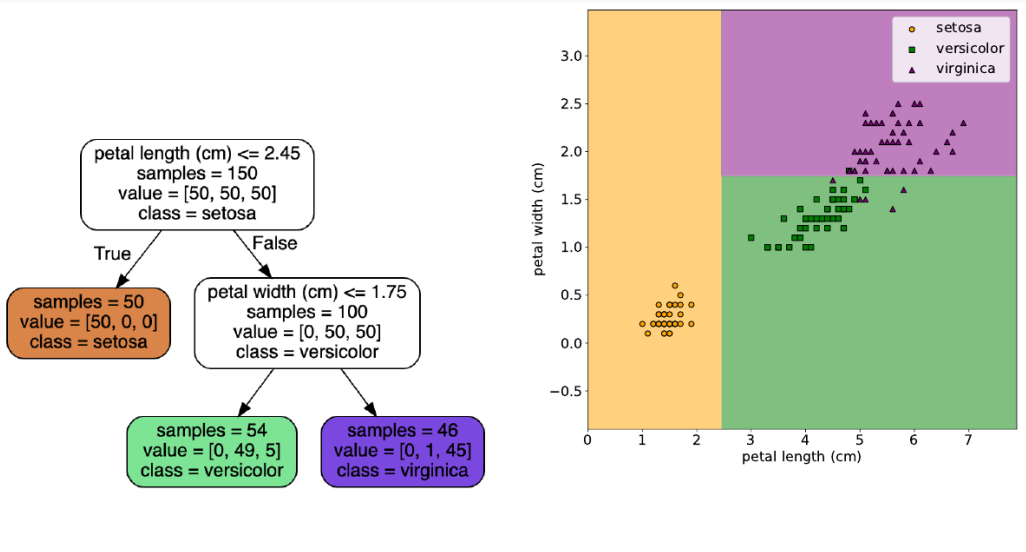
\includegraphics[width=0.98\textwidth]{Images/iris_decision_tree.PNG}
\caption{Decision tree per problema di classificazione specie di iris.}\label{fig:iris-decision-tree}
\end{figure}

\end{example}

\section{Richiami di probabilità}
Abbiamo diverse definizioni di probabilità.
\begin{description}
\item[Definizione Frequentistica] La probabilità di un evento è il rapporto tra il numero di casi favorevoli e il numero di casi possibili.
\item[Definizione Soggettiva] La probabilità di un evento è il prezzo che un individuo ritiene equo pagare per ricevere 1 se l'evento si verifica e 0 altrimenti.
\item[Definizione Bayesiana] La probabilità di un evento è l'\textit{incertezza} con cui l'evento si verifica.
\item[Definizione Assiomatica] Kolmogorov nel 1933 costruisce la teoria della probabilità a partire da degli assiomi.
\end{description}

L'incertezza può essere di due tipi:
\begin{description}
\item[aleatoria] ovvero è una \im{data uncertanty};
\item[epistemica] ovvero è una \im{model uncertanty};
\end{description}

\subsection{Proprietà della probabilità}
Chiamiamo $\pr(A)$ la probabilità dell'evento $A$, allora abbiamo le seguenti proprietà.

\begin{property}[Joint probability]
Se $A$ e $B$ sono due eventi indipendenti, allora:
\begin{equation}
\pr\pare{A\et B} \equiv \pr\pare{A, B} = \pr\pare{A} \cdot \pr\pare{B}.
\end{equation}
\end{property}

\begin{property}[Union probability]
Anche detta regola di unione esclusione. Se $A$ e $B$ sono due eventi indipendenti, allora:
\begin{equation}
\pr\pare{A\orr B} = \pr\pare{A} + \pr\pare{B} - \pr\pare{A\et B}.
\end{equation}
\end{property}

\begin{property}[Conditional probability]
\begin{equation}
\pr\pare{A\cond B} = \frac{\pr\pare{A, B}}{\pr\pare{A}}.
\end{equation}
Se i due eventi sono indipendenti questa si riduce a $\pr\pare{A\cond B} = \pr\pare{A}$.
\end{property}

\begin{property}[Conditional independece]
\begin{equation}
\pr\pare{A, B \cond C} = \pr\pare{A\cond C} \cdot \pr\pare{B\cond C}
\end{equation}
\end{property}

\subsection{Random variables}
Rappresentiamo con $X$ una variabile di cui non conosciamo il valore e la chiamiamo \textit{variabile casuale} (\im{random variable}). Il set dei valori che $X$ può assumere è detto \textit{spazio di sampling} (\im{sampling space}). Un evento è dunque un set di risultati dato un sampling space definito.

Se la variabile è \textbf{discreta} abbiamo un sampling space numerabile e la PMF (\im{probability mass function}):
\begin{equation}
p\pare{x} \equiv \pr\pare{X = x}.
\end{equation}
Se invece la variabile è \textbf{continua} abbiamo un samplig space non numberabile e la CDF (\im{cumulative distribution function}):
\begin{equation}
P\pare{x} \equiv \pr\pare{X \leq x},
\end{equation}
da cui possiamo definire la PDF (\im{probability density function}):
\begin{equation}
p\pare{x} \equiv \deriv{}{x}P\pare{x},
\end{equation}
da cui segue:
\begin{align}
&\pr\pare{a \leq X \leq b} = \int_a^b p\pare{x} = P\pare{b} - P\pare{a} \\
&\Longrightarrow \pr\pare{x \leq X \leq x + dx} \approx p\pare{x}.
\end{align}
Se la CDF $P\pare{x}$ è monotona crescente allora la sua inversa $P^{-1}(q)$ è detta \textit{quantile}. Il valore $x_q = P^{-1}\pare{q}$ è il valore per cui $\pr\pare{X\leq x_q} < q$, ovvero il quantile $q$ della distribuzione $P$.

Se abbiamo due variabili casuali $X$ e $Y$ allora possiamo definire la \im{joint distribution}:
\begin{equation}
p\pare{x, y} = p\pare{X = x, Y = y} \equiv p\pare{X = x\et Y = y}.
\end{equation}
Se le due variabili sono indipendenti e con cardinalità finita possiamo definire la \textit{distribuzione marginale} (\im{marginal distribution}) come:
\begin{equation}
p\pare{X = x} = \sum_y p\pare{X=x, Y=y},
\end{equation}
altrimenti se sono dipendenti la \textit{distribuzione condizionale} (\im{conditional distribution}) come:
\begin{equation}
\begin{split}
&p\pare{Y=y\cond X=x} = \frac{p\pare{X=x, Y=y}}{p\pare{X=x}} \\
&\Longrightarrow\quad p\pare{x, y} = p\pare{y\cond x}\cdot p\pare{x},
\end{split}
\end{equation}
da cui segue la \textbf{chain rule}:
\begin{equation}
p\pare{\vec{x}_{1,D}} = p\pare{x_1} p\pare{x_2\cond x_1} p\pare{x_3\cond x_1, x_2}\cdots p\pare{x_D\cond p_{1: D-1}}.
\end{equation}

Due variabili si dicono \im{marginalmente indipendenti} se
\begin{equation}
X\perp Y \quad\Longleftrightarrow\quad p\pare{X, Y} = p\pare{X} p\pare{Y},
\end{equation}
mentre si dicono \textbf{condizionalmente indipendenti} se
\begin{equation}
X\perp Y \quad\Longleftrightarrow\quad p\pare{X, Y\cond Z} = p\pare{X\cond Z} p\pare{Y\cond Z}. 
\end{equation}

\subsection{Momenti di una distribuzione}

\begin{definition}[Media] Definiamo \im{media} di una distribuzione come
\begin{equation}
\mathbb{E}\spare{X} \equiv \int_X x\, p\pare{x}dx \qquad\pare{ \mathbb{E}\spare{X_{\text{discreta}}} = \sum_{x\in X} x\, p\pare{x} }.
\end{equation}
La media è lineare, ovvero $\mathbb{E}\spare{\sum_{i=1}^n} = \sum_{i=1}^N \mathbb{E}\pare{X_i}$.
\end{definition}

\begin{definition}[Varianza] Definiamo \im{varianza} di una distribuzione come
\begin{equation}
\mathbb{V}\spare{X} \equiv \mathbb{E}\spare{\pare{X - \mu}^2},
\end{equation}
che con la definizione di prima possiamo anche scrivere come:
\begin{equation}
\begin{split}
\mathbb{V}\spare{X} &= \int_X \pare{x - \mu}^2\, p\pare{x}dx \\
&= \int x^2\, p\pare{x}dx \, +\, \mu^2\underbrace{\int p\pare{x}dx}_{=1} \, -\, 2\mu\underbrace{\int x\, p\pare{x}dx}_{=\mu} \\
&= \mathbb{E}\spare{X^2} - \mu^2.
\end{split}
\end{equation}
Con questa definizione è facile dimostrare l'identità
\begin{equation}
\mathbb{V}\spare{aX + b} = a^2\,\mathbb{V}\spare{X},
\end{equation}
inoltre anche la varianza è lineare, ma solo se le variabili sono indipendenti.
\end{definition}

\begin{definition}[Moda]
Definiamo \im{media} di una distribuzione il valore (o i valori) più probabile, ovvero
\begin{equation}
x^\star \;\text{t.c.}\; p\pare{x^\star} = \max p\pare{x},
\end{equation}
\end{definition}

Questi stimatori non danno tutta l'informazione contenuta nella distribuzione.

\subsection{Teorema di Bayes}

\begin{theorem}[Teorema di Bayes]\label{teo:bayes}
Data una quantità non nota $H$ (hypotesis) e dei dati noti $Y=y$ abbiamo che
\begin{equation}
p\pare{H=h\cond Y=y} = \frac{p\pare{H=h}p\pare{Y=y\cond H=h}}{p\pare{Y=y}}.
\end{equation}
\end{theorem}
Il teorema segue dall'identità $p\pare{h\cond y} p\pare{y} = p\pare{h} p\pare{y\cond h}$.
\begin{itemize}
\item $p\pare{h}$ viene detta \im{prior} ovvero ciò che conosciamo o assumiamo per $H$ \textit{prima} di fare qualunque misura;
\item $p\pare{y\cond h}$ è la \textit{distribuzione osservata} detta \im{likelihood}, è una funzione di $y$ ad $h$ fisso, ma non è un distribuzione di probabilità;
\item $p\pare{y}$ è detta \im{marginal likelihood}, indipendente da $h$, funge da costante di normalizzazione \[
p\pare{Y=y} = \sum_{h'\in H}p\pare{Y=y \cond H=h'} = \sum_{h'\in H}p\pare{H=h', Y=y};
\]
\item $p\pare{h\cond y}$ è detta \im{posterior distribution}.
\end{itemize}

\begin{example}[Monty Hall problem]
Posso scegliere una di tre porte. Dietro una delle porte c'è un premio. Inizio con il scegliere la porta 1. Ho che la probabilità degli eventi $H_{1,2,3}$ che il premio sia dietro la porta 1, 2 o 3 è
\[
p\pare{H_1} = p\pare{H=1} = \frac{1}{3}.
\]
Ora una delle porte non scelte da me si apre rivelando che dietro quella non c'è il premio, in base a dove si trova il premio la probabilità degli eventi $Y_{2, 3}$ che si apra una porta o l'altra è data da $p\pare{Y=y, H=h}$:
\[
\begin{array}{l@{,\qquad}l@{,\qquad}l}
p\pare{Y=2, H_1} = \frac{1}{2} & p\pare{Y=2, H_2} = 0 & p\pare{Y=2, H_3} = 1, \\
\\
p\pare{Y=3, H_1} = \frac{1}{2} & p\pare{Y=3, H_2} = 1 & p\pare{Y=3, H_3} = 1. \\
\end{array}
\]
Si apre la porta 3. Mi viene data la scelta di cambiare porta prima che venga rivelato dove si trova il premio, per massimizzare la probabilità di vittoria posso calcolare le probabilità condizionate con Bayes. Dai calcoli di prima ho che $p\pare(Y=3) = 1/6 + 1/3 = 1/3$ dunque:
\begin{equation}
\begin{split}
p\pare{H_1\cond Y=3} &= \dfrac{\frac{1}{3}\cdot\frac{1}{2}}{\frac{1}{2}} = \frac{1}{3}, \\
p\pare{H_2\cond Y=3} &= \dfrac{\frac{1}{3}\cdot 1}{\frac{1}{2}} = \frac{2}{3}, \\
p\pare{H_3\cond Y=3} &= 0, \\
\end{split}
\end{equation}
dunque mi conviene cambiare porta.
\end{example}

\subsection{Distribuzione di Gauss}
La distribuzione di Gauss (o gaussiana) è una tra le più usate in Machine Learning ed è definita come
\begin{equation}
\begin{split}
&P\pare{y} \equiv \pr\pare{Y\leq y},\qquad \pr\pare{a \leq Y \leq b} = P\pare{b} - \pare{a} \\
&\Phi\pare{y;\mu, \sigma^2} \equiv \int_{-\infty}^y \mathcal{N}\pare{\xi/\mu, \sigma^2}d\xi = \frac{1}{2}\spare{1 + \erf\pare{\frac{\xi}{\sqrt{2}}}},\quad \xi = \frac{y - \mu}{\sigma},
\end{split}
\end{equation}
ove $\erf$ è la \im{Gauss error function} definita come
\begin{equation}
\erf\pare{u} \equiv \frac{2}{\sqrt{\pi}} \int_0^\mu e^{-t^2}dt,
\end{equation}
mentre $\mathcal{N}$ è la PDF (probability density function) definita come
\begin{equation}
\mathcal{N}\pare{y\cond\mu,\sigma^2} \equiv \frac{1}{\sqrt{2\pi\sigma^2}}\exp\spare{-\frac{1}{2\sigma^2}\pare{y-\mu}^2}.
\end{equation}

Questa distribuzione è popolare per diversi motivi:
\begin{itemize}
\item dipende da soli due parametri ed entrambi sono di facile interpretazione;
\item per il teorema del limite centrale, nel limite $N\longrightarrow\infty$ ogni distribuzione può essere approssimata da una gaussiana;
\item rappresenta la somma di variabili causali indipendenti;
\item il numero di assunzioni è minimo.
\end{itemize}

\subsection{Altre distribuzioni notevoli}
Abbiamo:
\begin{itemize}
\item \im{t-Student} \begin{equation}
\tau\pare{y\cond\mu, \sigma^2, \nu} \propto \spare{1 + \frac{1}{\nu}\pare{\frac{y-\mu}{\sigma}}^2}^{-\frac{\nu+1}{2}}
\qquad\left\{\begin{array}{ll}
\mu & \text{mean} \\
\sigma & \text{mode} \\
\nu & \text{degree of formality} \\
\end{array}\right.;
\end{equation}
\item \im{Lorentz (Cauchy)} \begin{equation}
C\pare{x\cond\mu, \gamma} = \frac{1}{\gamma\pi}\spare{1 + \pare{\frac{x-\mu}{\gamma}}^2}^{-1};
\end{equation}
\item \im{Laplace} \begin{equation}
L\pare{y\cond\mu, b} = \frac{1}{2b}\exp\pare{-\frac{\left|y-\mu\right|}{b}}
\qquad\left\{\begin{array}{ll}
\mu & \text{mean} \\
\mu & \text{mode} \\
2b^2 & \text{variance} \\
\end{array}\right.;
\end{equation}
\item \im{beta} \begin{equation}
\Beta\pare{x\cond a, b} = \frac{1}{\beta\pare{a, b}}x^{a-1}\pare{1-x}^{b-1}
\qquad\left\{\begin{array}{ll}
\frac{a}{a+b} & \text{mean} \\
\pare{a-1}\pare{a+b-2} & \text{mode} \\
\frac{ab}{\pare{a+b}^2\pare{a+b+1}} & \text{variance} \\
\end{array}\right.;
\end{equation}
\item \im{gamma} \begin{equation}
\Ga\pare{x\cond a, b} = \frac{b^a}{\Gamma\pare{a}}x^{a-1}e^{-xb};
\end{equation}
\item \im{experimental} \begin{equation}
\Exp\pare{x\cond\lambda} = \Ga\pare{x\cond a=1, b=\lambda}
\end{equation}
\item \im{chi quadro} \begin{equation}
\chi^2_\nu\pare{x} = \Ga\pare{x\cond a=\frac{\nu}{2}, b=\frac{1}{2}}
\end{equation}
\end{itemize}
Alcune distribuzioni sono mostrate in \cref{fig:distributions}.

\begin{figure}
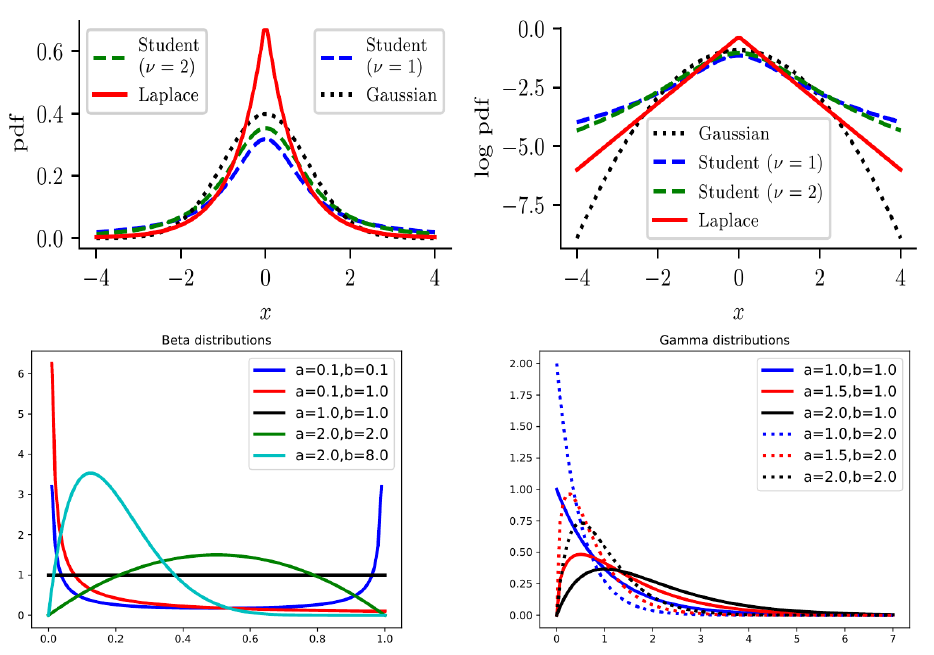
\includegraphics[width=0.98\textwidth]{Images/distributions.PNG}
\caption{Alcune distribuzioni notevoli.}\label{fig:distributions}
\end{figure}

\subsection{Osservazioni}
Supponiamo di avere due variabili causali descritte da distribuzioni gaussiane:
\begin{equation}
x_1 \sim \mathcal{N}\pare{\mu_1, \sigma_1^2},\qquad x_2 \sim \mathcal{N}\pare{\mu_2, \sigma_2^2},
\end{equation}
e di voler calcolare la PDF della loro somma $y = x_1 + x_2$, allora:
\begin{equation}
p\pare{y} = \mathcal{N}\pare{x_1\cond\mu_1, \sigma^2_1} \otimes \mathcal{N}\pare{x_2\cond\mu_2, \sigma^2_2} = \mathcal{N}\pare{y\cond\mu_1 + \mu_2, \sigma^2_1 + \sigma^2_2},
\end{equation}
ovvero \textit{la convoluzione di due gaussiane è una gaussiana}.

Supponiamo ora che $x$ sia una variabile casuale e $y = f\pare{x}$ una funzione di essa. Talora è difficile calcolare $p\pare{y}$ analiticamente. Supponiamo ad esempio che $x\sim\Unif\pare{-1,+1}$ e $y=x^2$, possiamo approssimare $p\pare{y}$ con un generatore (uniforme) di numeri casuali e facendone il quadrato per poi prendere la \im{distribuzione empirica}
\begin{equation}
p_S\pare{y} = \frac{1}{N_S}\sum_{x=1}^{N_S}\delta\pare{y-y_s}.
\end{equation}
Questo è detto \im{metodo monte carlo}.

\subsection{Modelli multivariati}
\begin{definition}[Covarianza]
Siano $X$ e $Y$ due variabili. La \im{covarianza} è
\begin{equation}
\Cov\spare{X, Y} \equiv \mathbb{E}\spare{\pare{X - \mathbb{E}\pare{E}}\pare{Y - \mathbb{E}\pare{E}}} = \mathbb{E}\spare{XY} - \mathbb{E}\spare{X}\mathbb{E}\spare{Y},
\end{equation}
ovvero una matrice $D$-dimensionale, con $D = \dim\pare{\vec{x}}$, che contiene le varianze sulla diagonale.
\end{definition}

\begin{definition}(Correlazione di Pearson)
La \im{correlazione di Pearson} tra le due variabili $X$ e $Y$ si definisce come
\begin{equation}
\rho \equiv \corr\spare{X, Y} = \frac{\Cov\spare{X, Y}}{\sqrt{\mathbb{V}\spare{X}\mathbb{V}\spare{Y}}}.
\end{equation}
\end{definition}

Possiamo scrivere
\begin{equation}
\Cov\spare{X} = \pare{\begin{array}{cccc}
\mathbb{V}\spare{X_1} & \Cov\spare{X_1, X_2} & \cdots & \Cov\spare{X_1, X_D} \\
\Cov\spare{X_2, X_1} & \mathbb{V}\spare{X_2} & \cdots & \Cov\spare{X_2, X_D} \\
\vdots & \vdots & \ddots & \vdots \\
\Cov\spare{X_D, X_1} & \Cov\spare{X_D, X_2} & \cdots & \mathbb{V}\spare{X_D} \\
\end{array}}
\end{equation}
e
\begin{equation}
\corr\pare{x} = \pare{\begin{array}{cccc}
1 & \frac{\mathbb{E}\spare{\pare{x_1-\mu_1}\pare{x_2-\mu_2}}}{\sigma_1\sigma_2} & \cdots & \frac{\mathbb{E}\spare{\pare{x_1-\mu_1}\pare{x_D-\mu_D}}}{\sigma_1\sigma_D} \\
\frac{\mathbb{E}\spare{\pare{x_2-\mu_2}\pare{x_1-\mu_1}}}{\sigma_2\sigma_1} & 1 & \cdots & \frac{\mathbb{E}\spare{\pare{x_2-\mu_2}\pare{x_D-\mu_D}}}{\sigma_2\sigma_D} \\
\vdots & \vdots & \ddots & \vdots \\
\frac{\mathbb{E}\spare{\pare{x_D-\mu_D}\pare{x_1-\mu_1}}}{\sigma_D\sigma_1} & \frac{\mathbb{E}\spare{\pare{x_D-\mu_D}\pare{x_2-\mu_2}}}{\sigma_D\sigma_2} & \cdots & 1 \\
\end{array}}.
\end{equation}

\subsubsection{Osservazioni}
\begin{itemize}
\item Il fatto che due variabili non siano correlate non vuol dire che siano indipendenti, tuttavia due variabili indipendenti sono necessariamente non correlate;
\item correlazione non implica causalità;
\item una correlazione che appare simile in diversi set di dati può sparire (o divenire opposta) se i dati sono combinati, questo è noto come \textit{Simpson's paradox}.
\end{itemize}

\subsection{Distribuzione gaussiana multivariata}
La definizione che abbiamo dato di distribuzione gaussiana si estende a più variabili. Innanzitutto definiamo la PDF
\begin{equation}
\mathcal{N}\pare{\vec{y}\cond\vec{\mu}, \Sigma} \equiv \frac{1}{\pare{2\pi}^{D/2}\left|\Sigma\right|^{1/2}}\exp\left\{-\frac{1}{2}\pare{\vec{y}-\vec{\mu}}^T\Sigma^{-1}\pare{\vec{y}-\vec{\mu}}\right\},
\end{equation}
dove $\Sigma = \Cov\spare{\vec{y}}$.

Supponiamo di avere due variabili aleatorie $\vec{y}_1$ e $\vec{y}_2$. Si può definire la distribuzione \im{jointly gaussian}. Con
\[
\vec{\mu} = \pare{\begin{array}{c}
\mu_1 \\
\mu_2
\end{array}},\qquad
\Sigma = \pare{\begin{array}{cc}
\Sigma_{11} & \Sigma_{12} \\
\Sigma_{21} & \Sigma_{22}
\end{array}},\qquad
\Lambda = \Sigma^{-1}
\]
le distribuzioni marginali sono
\begin{equation}
p\pare{\vec{y}_1} = \mathcal{N}\pare{\vec{y}_1\cond\vec{\mu}_1, \Sigma_{11}},\qquad p\pare{\vec{y}_2} = \mathcal{N}\pare{\vec{y}_2\cond\vec{\mu}_2, \Sigma_{22}}
\end{equation}
e la probabilità condizionata
\begin{equation}
p\pare{\vec{y}_1\cond\vec{y}_2} = \mathcal{N}\pare{\vec{y}_1\cond\vec{\mu}_{1\cond 2}, \Sigma_{1\cond 2}},
\end{equation}
con
\[
\vec{\mu}_{1\cond 2} = \vec{\mu}_1 + \Sigma_{12}\Sigma_{22}^{-1}\pare{\vec{y}_2 - \vec{\mu_2}},\qquad \Sigma_{1\cond 2} = \Sigma_{11} - \Sigma_{12}\Sigma_{22}^{-1}\Sigma_{21}=\Lambda_{11}^{-1},
\]
queste sono tutte gaussiane.

\section{Richiami di statistica}
Nella sezione precedente abbiamo assunto come noti i parametri $\vec{\theta}$, in questa sezione impariamo come è possibile imparare questi parametri a partire dai dati (training set) $\mathcal{D}$. Come abbiamo visto nell'\Cref{ex:iris}, il problema si riduce a trovare $\hat{\theta}$ tale che minimizzi il misclassification rate, \Cref{eq:misclassification-rate}, ovvero:
\[
\hat{\theta} \quad\text{t.c.}\quad \mathcal{L}(\hat{\theta}) = \min\spare{\mathcal{L}\pare{\theta}} \equiv \min\spare{\frac{1}{N}\sum_{n=1}^N l\pare{y_n, f\pare{\vec{x_n}, \vec{\theta}}}}.
\]

\subsection{Maximum likelihood estimation (MLE)}
\begin{definition}[Maximum likelihood estimation]
Definitiamo la MLE, \im{maximum likelihood estimation}, come il valore di $\theta$ che massimizza la probabilità condizionata di aver ottenuto il set di dati $\mathcal{D}$, ovvero:
\begin{equation}
\hat{\theta}_{\text{MLE}} \equiv \argmax_{\vec{\theta}} p\pare{\mathcal{D}\cond\vec{\theta}}.
\end{equation}
Se i dati sono campioni indipendenti della stessa distribuzione, allora possiamo anche scrivere
\begin{equation}
p\pare{\mathcal{D}\cond\vec{\theta}} = \prod_{n=1}^N p\pare{\vec{y}_n \cond \vec{x}_n, \vec{\theta}}.
\end{equation}
Definiamo inoltre la NLL, \textsc{negative log-likelihood}, da usare come loss function come:
\begin{equation}
l\pare{\vec{\theta}} \equiv -\log p\pare{\mathcal{D}\cond\vec{\theta}} = -\sum_{n=1}^N \log p\pare{\vec{y}_n \cond \vec{x}_n , \vec{\theta}}.
\end{equation}
\end{definition}

Con queste definizioni abbiamo che la MLE è data
\begin{itemize}
\item per supervised learning da:
\begin{equation}
\hat{\theta}_{\text{MLE}} = \argmin_{\vec{\theta}} -\sum_{n=1}^N \log p\pare{\vec{y}_n \cond \vec{x}_n, \vec{\theta}};
\end{equation}
\item per unsupervised learning da:
\begin{equation}
\hat{\theta}_{\text{MLE}} = \argmin_{\vec{\theta}} -\sum_{n=1}^N \log p\pare{\vec{y}_n \cond \vec{\theta}}.
\end{equation}
\end{itemize}

Possiamo giustificare l'uso della MLE pensandola come un'approssimazione del \textit{posterior} Bayesiano dato un \textit{prior} uniforme.

\begin{example}
Se abbiamo
\[
p\pare{\vec{\theta}\cond\mathcal{D}} = \delta\pare{\vec{\theta}- \hat{\theta}_{\text{MAP}}}
\]
con $\hat{\theta}$ il posterior, allora
\[
\hat{\theta}_{\text{MAP}} = \argmin_{\vec{\theta}}-\log p\pare{\vec{\theta}\cond\mathcal{D}} = \argmin_{\vec{\theta}} -\log p\pare{\mathcal{D}\cond\vec{\theta}} -\log p\pare{\vec{\theta}},
\]
ed essendo $p\pare{\vec{\theta}} = 1$ abbiamo
\[
\pushQED{\qed}
\hat{\theta}_{\text{MAP}} = \argmin_{\vec{\theta}} -\log p\pare{\mathcal{D}\cond\vec{\theta}} = \hat{\theta}_{\text{MLE}}.\qedhere
\popQED
\]
\end{example}

\subsubsection{Distribuzione normale}
Supponiamo ora di avere una variabile casuale $Y$ distribuita normalmente, i.e. $Y\sim \mathcal{N}\pare{\mu, \sigma^2}$, e sia $\mathcal{D} = \left\{ y_n \tc n=1,\cdots,N \right\}$ un dataset con punti campionati indipendentemente, allora:
\begin{equation}
\begin{split}
\NLL\pare{\mu, \sigma^2} &= -\sum_{n=1}^{N_D}\log\spare{\pare{\frac{1}{2\pi\sigma^2}}^\HALF \exp\pare{-\frac{1}{2\sigma^2}\pare{y_n-\mu}^2}} \\
&=\frac{1}{2\sigma}\sum_{n=1}^{N_D}\pare{y_n - \mu}^2 + \frac{N_D}{2}\log\pare{2\pi\sigma^2}.
\end{split}
\end{equation}
Ora estremizzando otteniamo
\begin{align}
\pderiv{}{\mu}\NLL\pare{\mu, \sigma^2} = 0 &\;\Longleftrightarrow\; \hat{\mu}_{\MLE} = \frac{1}{N_D}\sum_{n=1}^{N_D} y_n = \bar{y}\\
\pderiv{}{\sigma^2}\NLL\pare{\mu, \sigma^2} = 0 &\;\Longleftrightarrow\; \hat{\sigma}^2_\MLE = \frac{1}{N_D}\sum_{n=1}^{N_D}\pare{y_n - \hat{\mu}_\MLE}^2 = \frac{1}{N_D}\sum_{n=1}^{N_D}y_n^2 - \bar{y}^2 = s^2 - \bar{y}^2.
\end{align}

\subsubsection{Distribuzione normale multivariata}
Per una distribuzione multivariata i risultati sono analoghi. Abbiamo
\begin{equation}
l\pare{\vec{\mu}, \Sigma} = \log p\pare{\mathcal{D}\cond\vec{\mu},\Sigma} = \frac{N_D}{2}\log\left|\Lambda\right| = -\HALF\sum_{n=1}^{N_D}\pare{\vec{y}_n - \vec{\mu}}^T \Lambda\pare{\vec{y}_n - \vec{\mu}}
\end{equation}
dove $\Lambda = \Sigma^{-1}$ è la \im{precision matrix}. Dall'estremizzazione segue, come prima, l'empirical mean $\hat{\vec{\mu}}$ e l'empirical covariance matrix $\hat{\Sigma}$:
\begin{align}
\hat{\vec{\mu}} &= \frac{1}{N_D}\sum_{n=1}^{N_D}\vec{y_n} = \bar{\vec{y}} \\
\hat{\Sigma} &= \frac{1}{N_D}\sum_{n=1}^{N_D}\pare{\bar{\vec{y}}_n - \bar{\vec{y}}}\pare{\bar{\vec{y}}_n - \bar{\vec{y}}}^T 
\end{align}

\subsection{Empirical risk minimization (ERM)}
La MLE può essere generalizzata sostituendo la loss function logaritmica NLL con qualunque altra funzione $l$:
\begin{equation}
\mathcal{L}\pare{\vec{\theta}} = \frac{1}{N}\sum_{n=1}^N l\pare{\vec{y}_n, \vec{\theta}; \vec{x}_n}.
\end{equation}
Questo processo di cambiare loss function è noto come ERM, \im{empirical risk minimization}. %% ???

\begin{example}[ERM per problema di classificazione]
In un problema di classificazione avremo una loss function
\begin{equation}
l_{01}\pare{\vec{y}_n, \vec{\theta}; \vec{x}_n} = \left\{\begin{array}{l@{\quad\text{se}\quad}l}
1 & \vec{y}_n = f\pare{\vec{x}_n; \vec{\theta}} \\
0 & \vec{y}_n \neq f\pare{\vec{x}_n; \vec{\theta}} 
\end{array}\right.
\end{equation}
dove $f\pare{\vec{x}, \vec{\theta}}$ è un predittore. L'empirical risk diviene
\begin{equation}
\mathcal{L}\pare{\vec{\theta}} = \frac{1}{N}\sum_{n=1}^N l_{01}\pare{\vec{y}_n, \vec{\theta}; \vec{x}_n},
\end{equation}
che è il misclassification rate nel training set. In problemi binari possiamo riscrivere il misclassification rate usando l'indicatore binario come definito in \eqref{eq:indicatore-binario}. Se $\tilde{y} \in \left\{ -1, +1 \right\}$ è il time label e $\hat{y}\in \left\{-1, +1\right\} = f\pare{\vec{x}, \vec{\theta}}$ la prediction, allora:
\begin{equation}
l_{01}\pare{\tilde{y}, \hat{y}} = \mathbb{I}\pare{\tilde{y}\neq\hat{y}} = \mathbb{I}\pare{\tilde{y}\hat{y}<0},
\end{equation}
con cui il rischio empirico si scrive
\begin{equation}
\mathcal{L}\pare{\vec{\theta}} = \frac{1}{N}\sum_{n=1}^{N}l_{01}\pare{\tilde{y}_n, \hat{y}_n} = \frac{1}{N}\sum_{n=1}^N\mathbb{I}\pare{\tilde{y}_n\hat{y}_n < 0}.
\end{equation}
La funzione $l_{01}$ è però problematica in quanto non-smooth e quindi difficile da ottimizzare. In questi casi si può utilizzare una funzione surrogata, definita generalmente come limite superiore convesso, ad esempio
\begin{equation}
l_{ll}\pare{\tilde{y}, \eta} = -\log{p\pare{\tilde{y}\cond\eta}} = \log\pare{1 + e^{-\tilde{y}\eta}},\qquad p\pare{\tilde{y}\cond\vec{x},\vec{\theta}} = \sigma\pare{\hat{y}\eta} = \frac{1}{1+e^{-\hat{y}\eta}}
\end{equation}
\end{example}

\subsection{Altri metodi di minimizzazione}

\subsubsection{Metodo dei momenti}
Il calcolo di $\nabla_{\vec{\theta}}\NLL\pare{\vec{\theta}} = 0$, ovvero la ricerca dei punti estremi, può essere difficile. Il metodo dei momenti consiste nell'eguagliare i momenti teorici della distribuzione ai momenti empirici, ovvero:
\begin{equation}
\left.
\begin{array}{ll}
\textsc{Momenti teorici:} & \mu_k = \mathbb{E}\spare{Y^k} \\
\\
\textsc{Momenti empirici:} & \hat{\mu}_k = \frac{1}{N}\sum_{n=1}^N y_n^k
\end{array}
\right\} \mu_k = \hat{\mu}_k \quad\Longrightarrow\quad \text{ho } k \text{ equazioni}.
\end{equation}
Ad esempio per la gaussiana abbiamo:
\begin{align*}
&\mu_1 = \mu = \bar{y}, \\
&\mu_2 = \sigma^2 + \mu^2 = s^2.
\end{align*}
In questo caso abbiamo che MOM $=$ MLE, ma questo non è vero in generale (ad esempio non è vero per la distribuzione uniforme).

\subsubsection{Online recursive estimation}
Se tutto il dataset $\mathcal{D}$ è noto e disponibile prima che inizi il processo di learning si dice che si fa \im{batch learning}. In alcuni casi però il dataset è disponibile in blocchi e si dice che si fa \im{online learning}. Si ha che $\hat{\vec{\theta}}_{t-1}$ è la predizione dato il blocco $\mathcal{D}_{1:t-1}$, quello che vogliamo fare è trovare $\vec{\theta}_t = f(\hat{\vec{\theta}}_{t-1}, \vec{y}_t)$ con un update ricorsivo.

\begin{definition}[Moving average]
Per una gaussiana multivariata si può definire la \im{media mobile} come:
\begin{equation}
\begin{split}
\hat{\vec{\mu}}_t &= \frac{1}{t}\sum_{n=1}^t\vec{y}_n \\
&= \frac{1}{t}\spare{\pare{t-1}\hat{\vec{\mu}}_{t-1} + \vec{y}_t} = \hat{\vec{\mu}}_{t-1} + \frac{1}{t}\pare{\vec{y}_t - \hat{\vec{\mu}}_{t-1}}.
\end{split}
\end{equation}
Nel caso in cui la distribuzione cambi in modo continuo la moving average può anche essere pesata.
\end{definition}

\subsection{Regolarizzazione}
Un problema della MLE (maximum likelihood estimation) e della ERM (empirical risk minimization) è che i parametri tendono ad essere determinati minimizzando il loss nel training set, ma non necessariamente lo minimizzano per i dati futuri. Per ridurre l'entità del problema si può procedere con la regolarizzazione:
\begin{equation}
\mathcal{L}\pare{\vec{\theta}, \lambda} = \Bigl[ \underbrace{\frac{1}{N}\sum_{n=1}^N l\pare{\vec{y}_n, \vec{\theta}; \vec{x}_n}}_{\mathcal{L}\pare{\vec{\theta}}} + \lambda C\pare{\vec{\theta}} \Bigr],
\end{equation}
dove $\lambda$ è detto \im{regularization parameter} e $C\pare{\vec{\theta}}$ è la \im{penality function}, ad esempio si può avere:
\[
C\pare{\vec{\theta}} = -\log{p\pare{\vec{\theta}}}.
\]

Per $\lambda = 1$ e riscalando $p\pare{\vec{\theta}}$ si ha la NLL:
\begin{equation}
\NLL\pare{\vec{\theta}, \lambda} = - \spare{\sum_{n=1}^N\log{p\pare{\vec{y}_n\cond\vec{x}_n,\vec{\theta}}} + \log{p\pare{\vec{\theta}}}} = -\spare{\log{p\pare{\mathcal{D}\cond\vec{\theta}}} + \log{p\pare{\vec{\theta}}}},
\end{equation}
che implica:
\begin{equation}
\hat{\vec{\theta}} = \argmax_{\vec{\theta}}\log{p\pare{\vec{\theta}\cond\mathcal{D}}} = \argmax_{\vec{\theta}}\spare{\log{p\pare{\mathcal{D}\cond\vec{\theta}}} + \log{p\pare{\vec{\theta}}} - \text{const}}.
\end{equation}
Questa stima si chiama MAP (\im{maximum a posterior}) estimation.


\subsubsection{Come scegliere $\lambda$}
Un valore (troppo) piccolo per $\lambda$ equivale a minimizzare il rischio empirico (\im{overfitting}); un valore (troppo) grande equivale a essere troppo vicini al prior (\im{underfitting}). Una soluzione è dividere il training set in due classi: una di training ($\mathcal{D}_{\text{train}},\,80\%$) ed una di validation ($\mathcal{D}_{\text{val}},\,20\%$). Si va quindi a fittare il modello su $\mathcal{D}_{\text{train}}$ per ogni setting $\lambda$ e poi a valutare la performance del modello ottenuto su $\mathcal{D}_{\text{val}}$. Si prende dunque il valore di $\lambda$ per cui si è ottenuta la performance migliore.

\begin{definition}[Regularized empirical risk]
Definiamo l'\im{empirical risk regolarizzato} come:
\begin{equation}
R_\lambda\pare{\vec{\theta}, \mathcal{D}} \equiv \frac{1}{\left|\mathcal{D}\right|}\sum_{\pare{\vec{x}, \vec{y}}\in\mathcal{D}} l\pare{\vec{y}, f\pare{\vec{x}, \vec{\theta}}} + \lambda C\pare{\theta}
\end{equation}
\end{definition}
\noindent
Il processo che seguiamo è quindi il seguente:
\begin{enumerate}
\item costruiamo il modello: $\hat{\vec{\theta}}_\lambda\pare{\mathcal{D}_\text{train}} = \argmin_{\vec{\theta}} R_\lambda\pare{\vec{\theta}, \mathcal{D}_{\text{train}}}\;\forall\lambda$;
\item calcoliamo il validation risk: $R_\lambda^\text{val} = R_0\pare{\hat{\vec{\theta}}_\lambda\pare{\mathcal{D}_\text{train}}, \mathcal{D}_\text{val}}$;
\item prendiamo il $\lambda$ che ha dato la miglior performance: $\lambda^\star = \argmin_{\lambda\in S} R_\lambda^\text{val}$;
\item si ri-fitta il modello su $\mathcal{D} = \mathcal{D}_\text{train}\cup\mathcal{D}_\text{val}$ usando $\lambda=\lambda^\star$;
\item si ottengono i parametri $\hat{\vec{\theta}}^\star = \argmin_{\vec{\theta}} R_{\lambda^\star}\pare{\vec{\theta}, \mathcal{D}}$.
\end{enumerate}

Se il dataset è piccolo, eliminare il $20\%$ dei dati può essere dannoso e si procede quindi con la \im{cross validation}. Questa consiste nel dividere il dataset in $K$ \im{fold} e per ognuno allenare il modello su tutti i fold meno il $k$-esimo, il quale viene usato come test fold. Si definisce l'empirical risk regolarizzato per cross validation:
\begin{equation}
R_\lambda^\text{CV} \equiv \frac{1}{K}\sum_{k=1}^K R_0\pare{\hat{\vec{\theta}}_\lambda\pare{\mathcal{D} - \mathcal{D}_k}, \mathcal{D}_k}
\end{equation}

\subsection{Statistica Bayesiana}
Abbiamo ora visto diversi metodi per determinare i parametri a partire dei dati, ma dobbiamo ancora parlare della loro incertezza. Il \Crefn{teo:bayes} ci aiuta in questo, infatti:
\begin{equation}
    p\pare{\vec{\theta}\cond \mathcal{D}} = \frac{p\pare{\vec{\theta}} p\pare{\mathcal{D}\cond\vec{\theta}}}{p\pare{\mathcal{D}}} = \frac{p\pare{\vec{\theta}} p\pare{\mathcal{D}\cond\vec{\theta}}}{\int p\pare{\vec{\theta}'}p\pare{\mathcal{D}\cond\vec{\theta}'}d\vec{\theta}'}
\end{equation}
\end{document}
